\documentclass[aspectratio=169]{beamer}
\usepackage{lectureppt} % Load your custom style
\usetikzlibrary{decorations.pathreplacing}


\title{수리경제학}
\subtitle{미분}
\author{이재석}
\date{2025-04-29 \\ (updated:\today)}

\begin{document}

\begin{frame}
  \titlepage
\end{frame}

\begin{frame}{목차}
  \tableofcontents
\end{frame}


%%%%%%%%%%%%%%%%%%%%%%%%%%%%%%%%%%%%%
%%%%%%%%%%%%%%%%%%%%%%%%%%%%%%%%%%%%%
% 
% 기본미분법칙
%  
%%%%%%%%%%%%%%%%%%%%%%%%%%%%%%%%%%%%%
%%%%%%%%%%%%%%%%%%%%%%%%%%%%%%%%%%%%%
\begin{frame}{미분의 정의와 의미}
  \begin{definition}[도함수]
    실수($\mathbb{R}$)의 어떤 함수 \textcolor{violet}{$f(x)$}가 정의되는 포인트 \textcolor{blue}{\emph{$a$}} 에서 \emph{미분가능(differentiable)} 하고, 정의역이 포인트 \textcolor{blue}{\emph{$a$}} 를 포함한다면, \textcolor{blue}{\emph{$a$}} 에서 \textcolor{red}{미분계수(순간변화율)} \textcolor{red}{\emph{$L$}} 은 \\
    \begin{equation}
      \textcolor{red}{L} = \textcolor{teal}{\lim_{h \to 0} \frac{f(\textcolor{blue}{a}+h)-f(\textcolor{blue}{a})}{h}}
    \end{equation}
  \end{definition}
  \begin{itemize}
    \item 미분하다: 함수 \textcolor{violet}{$f(x)$} 의 \textcolor{teal}{도함수}에 \textcolor{blue}{\emph{$x_0$}} 를 대입하여, \textcolor{red}{미분계수 $L$}의 값을 찾는다
    \item 어떤 함수 \textcolor{violet}{$f(x)$}를 미분하다 \\
    = \textcolor{violet}{$f(x)$} 의 \textcolor{red}{미분계수}를 구하다 \\
    = \textcolor{teal}{$f'(x \mid \textcolor{blue}{x = x_0})$}
    = \textcolor{teal}{$f'(x)$}를 구하다 \\
    = \textcolor{violet}{$f(x)$} 의 \textcolor{teal}{도함수}를 구하다 
    = \textcolor{teal}{$\frac{\mathbf{d}y}{\mathbf{d}x}$}
  \end{itemize}
\end{frame}




% 함수형태에 따른 도함수
% \section{주요 함수형태의 미분}
%%%%%%%%%%%%%%%%%%%%%%%%%%%%%%%%%%%%%
% Sec. polynomial, Cobb-Doug
%   * fraction, linear
%%%%%%%%%%%%%%%%%%%%%%%%%%%%%%%%%%%%%

\section{Power Rule}

\begin{frame}{함수에 따른 미분법: Power Rule}
  \begin{block}{상수함수의 미분법칙}
    \begin{align*}
      \frac{\mathbf{d}}{\mathbf{d}x} c = 0 , \quad C \text{ 는 상수 (constant)}
    \end{align*}
  \end{block}
  % 
  \begin{block}{Polynomial 미분: Power Rule}
    \begin{align*}
      \frac{\mathbf{d}}{\mathbf{d}x} x^n = n \cdot x^{n-1} 
    \end{align*}
  \end{block}
\end{frame}


\begin{frame}{함수에 따른 미분법: Polynomial $f(x) = ax$}
  \begin{definition}[도함수]
    % 실수($\mathbb{R}$)의 어떤 함수 \textcolor{violet}{$f(x)$}가 정의되는 포인트 \textcolor{blue}{\emph{$x_0$}} 에서 \emph{미분가능(differentiable)} 하고, 정의역이 포인트 \textcolor{blue}{\emph{$x_0$}} 를 포함한다면, \textcolor{blue}{\emph{$x_0$}} 에서 \textcolor{red}{미분계수(순간변화율)} \textcolor{red}{\emph{$L$}} 은 \\
    \begin{equation*}
      \textcolor{red}{L} = \textcolor{teal}{\lim_{h \to 0} \frac{f(\textcolor{blue}{x_0}+h)-f(\textcolor{blue}{x_0})}{h}}
    \end{equation*}
  \end{definition}
  % 
  \begin{align*}
    & \textcolor{magenta}{f(x) = ax}, \quad \text{도함수: } f'(x) = \lim_{h \to 0} \frac{f(x+h)-f(x)}{h} \\
    & \text{도함수에 대입. 예를 들어, } \textcolor{magenta}{f(x+h) = a(x+h)} \\
    & \rightarrow f'(x) = \lim_{h \to 0} \frac{\textcolor{magenta}{a(x+h)}- \textcolor{magenta}{ax}}{h} \\
    \lim \text{계산} \rightarrow & = \lim_{h \to 0} \frac{ax + ah -ax}{h} = \lim_{h \to 0} \frac{ah}{h} = \lim_{h \to 0} a = a\\
  \end{align*}
  % 
\end{frame}


\begin{frame}{함수에 따른 미분법: Polynomial $f(x) = ax^2$}
  \begin{align*}
    & \textcolor{magenta}{f(x) = ax^2}, \quad \text{도함수: } f'(x) = \lim_{h \to 0} \frac{f(x+h)-f(x)}{h} \\
    & \text{도함수에 대입} \rightarrow f'(x) = \lim_{h \to 0} \frac{\textcolor{magenta}{a(x +h)^2} - \textcolor{magenta}{ax^2}}{h} \\
    & = \lim_{h \to 0} \frac{ax^2 + 2axh + ah^2 - ax^2}{h} \\
    & = \lim_{h \to 0} \frac{2axh + ah^2}{h} = \lim_{h \to 0} 2ax + \lim_{h \to 0} ah = 2ax + a \cdot 0 = 2ax \\
    & \therefore f'(x) = 2ax \\
    & f'(x \mid x=1) = 2a\cdot 1, \quad f'(x \mid x=2) = 4a
  \end{align*}
  % 
\end{frame}

\begin{frame}{함수에 따른 미분법: Polynomial $f(x) = \frac{1}{x}, f(x) = x^{-1}$}
  \begin{align*}
    & f(x) = \textcolor{magenta}{\frac{1}{x}} = x^{-1}, \quad \text{도함수:} f'(x) = \lim_{h \to 0} \frac{f(x+h)-f(x)}{h} \\
    & \text{도함수에 대입} \rightarrow f'(x) = \lim_{h \to 0} \frac{ \textcolor{magenta}{\frac{1}{x+h}} - \textcolor{magenta}{\frac{1}{x}}}{h} \\
    & = \lim_{h \to 0} \frac{\frac{x - (x + h)}{x(x+h)}}{h}  = \lim_{h \to 0} \frac{\frac{-h}{x(x+h)}}{h} = \lim_{h \to 0} \frac{-h}{hx(x+h)}   \\
    & = \lim_{h \to 0} \frac{-1}{x(x+h)} = \lim_{h \to 0} \frac{-1}{x^2+hx}   = \frac{-1}{x^2} \\
    & \therefore f'(x) = -\frac{1}{x^2} = {-1}x^{-2} \\
    & f'(x \mid x=1) = -1, \quad f'(x \mid x=2) = -\frac{1}{4}
  \end{align*}
\end{frame}



\begin{frame}{다항함수와 도함수 비교: \(f(x) = x^2\), \(g(x) = x^3\), \(h(x) = \sqrt{x}\)}
  \scriptsize
  \begin{columns}
    % Left column: functions
    \begin{column}{0.5\textwidth}
      \centering
      \textbf{원 함수들}

      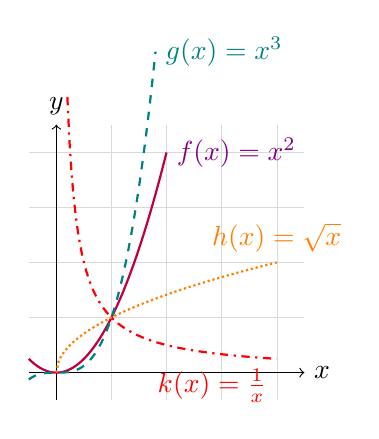
\begin{tikzpicture}[scale=0.7]
        % Grid
        \draw[step=1cm,gray,very thin,opacity=0.3] (-0.5,-0.5) grid (4.5,4.5);
      
        % Axes
        \draw[->] (-0.5,0) -- (4.5,0) node[right] {$x$};
        \draw[->] (0,-0.5) -- (0,4.5) node[above] {$y$};

        % f(x) = x^2
        \draw[thick,purple,domain=-0.5:2,samples=100] plot(\x,{\x*\x}) node[right] {\textcolor{violet}{$f(x) = x^2$}};
        
        % g(x) = x^3
        \draw[thick,teal,dashed,domain=-0.5:1.8,samples=100] plot(\x,{\x*\x*\x}) node[right] {\textcolor{teal}{$g(x) = x^3$}};

        % h(x) = sqrt(x)
        \draw[thick,orange,densely dotted,domain=0:4,samples=100] plot(\x,{sqrt(\x)}) node[above] {\textcolor{orange}{$h(x) = \sqrt{x}$}};

        % k(x) = 1/x
        \draw[thick,red,dashdotted,domain=0.2:4,samples=100] plot(\x,{1/\x}) node[below left] {\textcolor{red}{$k(x) = \frac{1}{x}$}};

      \end{tikzpicture}
    \end{column}

    % Right column: derivatives
    \begin{column}{0.5\textwidth}
      \centering
      \textbf{도함수들}

      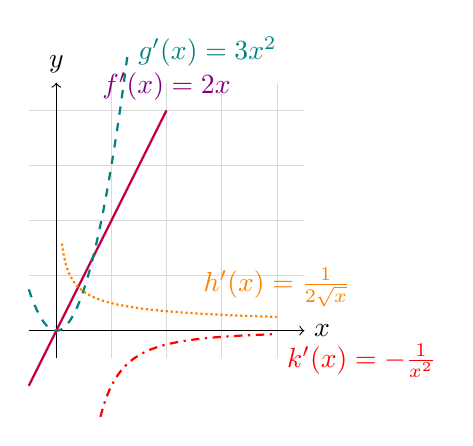
\begin{tikzpicture}[scale=0.7]
        % Grid
        \draw[step=1cm,gray,very thin,opacity=0.3] (-0.5,-0.5) grid (4.5,4.5);
      
        % Axes
        \draw[->] (-0.5,0) -- (4.5,0) node[right] {$x$};
        \draw[->] (0,-0.5) -- (0,4.5) node[above] {$y$};

        % f'(x) = 2x
        \draw[thick,purple,domain=-0.5:2,samples=100] plot(\x,{2*\x}) node[above] {\textcolor{violet}{$f'(x) = 2x$}};
        
        % g'(x) = 3x^2
        \draw[thick,teal,dashed,domain=-0.5:1.3,samples=100] plot(\x,{3*\x*\x}) node[right] {\textcolor{teal}{$g'(x) = 3x^2$}};

        % h'(x) = 1/(2*sqrt(x))
        \draw[thick,orange,densely dotted,domain=0.1:4,samples=100] plot(\x,{1/(2*sqrt(\x))}) node[above] {\textcolor{orange}{$h'(x) = \frac{1}{2\sqrt{x}}$}};

        % k'(x) = -1/x^2
        \draw[thick,red,dashdotted,domain=0.8:4,samples=100] plot(\x,{-1/(\x*\x)}) node[below right] {\textcolor{red}{$k'(x) = -\frac{1}{x^2}$}};

      \end{tikzpicture}
    \end{column}
  \end{columns}
\end{frame}



\begin{frame}%{함수에 따른 미분법: Polynomial 예제}
  \begin{align*}
    & f(x) = a \cdot x^2      & f'(x) = \hspace{4cm} & f''(x) = \hspace{4cm} \\[2em]
    & f(x) = \cdot x^{(-1/2)}   & f'(x) = \hspace{4cm} & f''(x) = \hspace{4cm} \\[2em]
    & f(x) = 2 \cdot x^2 + x  & f'(x) = \hspace{4cm} & f''(x) = \hspace{4cm} \\[2em]
  \end{align*}
\end{frame}







\section{지수함수 미분}
%%%%%%%%%%%%%%%%%%%%%%%%%%%%%%%%%%%%%
% Sec. exponential
% 
%%%%%%%%%%%%%%%%%%%%%%%%%%%%%%%%%%%%%
\begin{frame}{도함수의 정의로 미분:지수함수 미분법칙}
  \begin{block}{지수함수의 미분법칙}
    \begin{align*}
      & \frac{d}{dx} e^x = e^x \\
      & \frac{d}{dx} a^x = a^x \cdot \ln a   
    \end{align*}
  \end{block}
  \begin{align*}
    & f(x) = e^x \qquad \rightarrow \qquad f'(x) = e^x \\
    & f(x) = a^x \qquad \rightarrow \qquad  f'(x) = a^x \cdot \ln a
  \end{align*}
\end{frame}

\begin{frame}{도함수의 정의로 미분 - 지수함수}
  \begin{align*}
    f(x) & = e^x, \quad \text{도함수에 대입} \rightarrow  f'(x) = \lim_{h \to 0} \frac{f(x+h)-f(x)}{h} \\
    % & \text{도함수에 대입} \rightarrow \\
    f'(x) & = \lim_{h \to 0} \frac{e^{x+h} - e^x}{h} = \lim_{h \to 0} \frac{e^x \cdot e^h - e^x}{h} \\
    & = \lim_{h \to 0} \frac{e^x (e^h - 1)}{h} = e^x \cdot \lim_{h \to 0} \frac{\textcolor{blue}{e^h} - 1}{h} \\
    & \quad \quad \textcolor{blue}{e^h} \text{ 의 정의 } \textcolor{blue}{e^h = 1 + \frac{h}{1!} + \frac{h^2}{2!} + \cdots} \text{ 를 활용하여 대입하면,}\\
    & = e^x \cdot \lim_{h \to 0} \frac{\textcolor{blue}{1 + \frac{h}{1!} + \frac{h^2}{2!} + \cdots} - 1}{h}  = e^x \cdot \lim_{h \to 0} (\frac{h}{1!}/h + \frac{h^2}{2!}/h + \cdots) \\
    & = e^x \cdot (1 + 0 + \cdots) = e^x    
  \end{align*}
\end{frame}


\begin{frame}{도함수의 정의로 미분 - 지수함수}
  \scalebox{0.85}{%
  \parbox{\linewidth}{%
  \begin{align*}    
    f(x) & = a^x, \text{도함수에 대입} \rightarrow \\
    f'(x) & = \lim_{h \to 0} \frac{a^{x+h} - a^x}{h} = \lim_{h \to 0} \frac{a^x \cdot a^h - a^x}{h} 
    = \lim_{h \to 0} \frac{a^x (a^h - 1)}{h} = a^x \cdot \lim_{h \to 0} \frac{\textcolor{blue}{a^h} - 1}{h} \\
    & \quad \quad e^{\ln x} = x \text{의 성질을 이용하여 } a = e^{\ln a} \\
    & \quad \quad \text{양변을 h 거듭제곱하면, 로그의 성질에 의해 } \Rightarrow \textcolor{blue}{a^h} = \textcolor{blue}{e^{h \ln a}} \\
    & \quad \quad e \text{ 의 정의를 활용하기 위해, 양변에 1을빼고 h로 나누면, } \Rightarrow \frac{\textcolor{blue}{a^h} - 1}{h} = \frac{\textcolor{blue}{e^{h \ln a}} - 1}{h} \\
    & \quad \quad  \textcolor{teal}{h\ln a = u} \text{ 로 치환하고 정리하면, } \textcolor{olive}{h = \frac{u}{\ln a}}, \quad \frac{\textcolor{blue}{e^{h \ln a}} - 1}{\textcolor{olive}{h}} = \frac{\textcolor{teal}{e^u} - 1}{\textcolor{olive}{\frac{u}{\ln a}}} = \frac{\textcolor{teal}{e^u} - 1}{\textcolor{olive}{u}} \cdot \textcolor{olive}{\ln a} \\
    & \quad \quad  \text{이때, 극한은 $u$에 대해서로 변함: } \lim_{h \to 0} \textcolor{teal}{h\ln a} = 0 \text{ 이므로 } u \to 0 \\
    & = a^x \cdot \lim_{u \to 0} \frac{\textcolor{teal}{e^u} -1}{\textcolor{olive}{u}} \cdot \textcolor{olive}{\ln a} = a^x \cdot 1 \cdot \ln a \quad \quad (\because \lim_{h \to 0} \frac{{e^h} - 1}{h} = 1 \text{ 앞에서 찾음!})
  \end{align*}
  }%
  }
\end{frame}






% 지수함수 비교
\begin{frame}{지수함수와 도함수 비교: \(f(x) = 2^x\), \(g(x) = e^x\), \(h(x) = 3^x\)}
  \scriptsize
  \begin{columns}
    % Left column: functions
    \begin{column}{0.5\textwidth}
      \centering
      \textbf{원 함수들}

      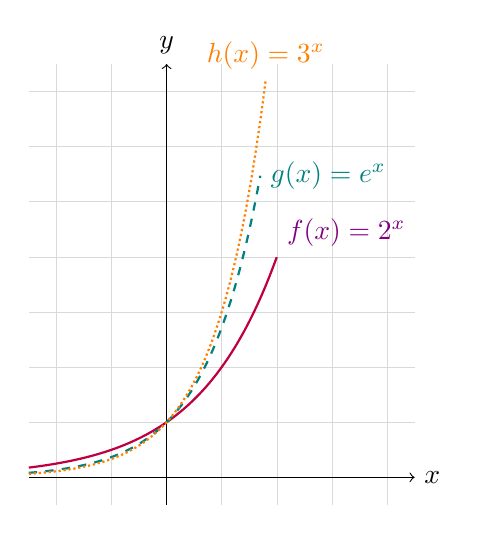
\begin{tikzpicture}[scale=0.7]
        % Grid
        \draw[step=1cm,gray,very thin,opacity=0.3] (-2.5,-0.5) grid (4.5,7.5);
      
        % Axes
        \draw[->] (-2.5,0) -- (4.5,0) node[right] {$x$};
        \draw[->] (0,-0.5) -- (0,7.5) node[above] {$y$};

        % f(x) = 2^x
        \draw[thick,purple,domain=-2.5:2,samples=100] plot(\x,{pow(2,\x)}) node[above right] {\textcolor{violet}{$f(x) = 2^x$}};
        
        % g(x) = e^x
        \draw[thick,teal,dashed,domain=-2.5:1.7,samples=100] plot(\x,{exp(\x)}) node[right] {\textcolor{teal}{$g(x) = e^x$}};

        % h(x) = 3^x
        \draw[thick,orange,densely dotted,domain=-2.5:1.8,samples=100] plot(\x,{pow(3,\x)}) node[above] {\textcolor{orange}{$h(x) = 3^x$}};
      \end{tikzpicture}
    \end{column}

    % Right column: derivatives
    \begin{column}{0.5\textwidth}
      \centering
      \textbf{도함수들}

      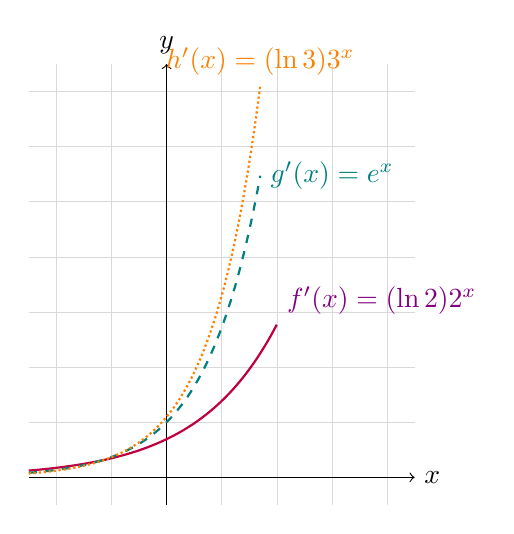
\begin{tikzpicture}[scale=0.7]
        % Grid
        \draw[step=1cm,gray,very thin,opacity=0.3] (-2.5,-0.5) grid (4.5,7.5);
      
        % Axes
        \draw[->] (-2.5,0) -- (4.5,0) node[right] {$x$};
        \draw[->] (0,-0.5) -- (0,7.5) node[above] {$y$};

        % f'(x) = 2^x * ln(2)
        \draw[thick,purple,domain=-2.5:2,samples=100] plot(\x,{ln(2)*pow(2,\x)}) node[above right] {\textcolor{violet}{$f'(x) = (\ln 2)2^x$}};
        
        % g'(x) = e^x
        \draw[thick,teal,dashed,domain=-2.5:1.7,samples=100] plot(\x,{exp(\x)}) node[right] {\textcolor{teal}{$g'(x) = e^x$}};

        % h'(x) = 3^x * ln(3)
        \draw[thick,orange,densely dotted,domain=-2.5:1.7,samples=100] plot(\x,{ln(3)*pow(3,\x)}) node[above] {\textcolor{orange}{$h'(x) = (\ln 3)3^x$}};
      \end{tikzpicture}
    \end{column}
  \end{columns}
\end{frame}

\begin{frame}
  \begin{align*}
    & f(x) = 2\cdot e^x & f'(x)= \hspace{4cm} & f''(x)= \hspace{4cm}\\[2em]
    & f(x) = e^x        & f'(x)= \hspace{4cm} & f''(x)= \hspace{4cm}
  \end{align*}
\end{frame}





%%%%%%%%%%%%%%%%%%%%%%%%%%%%%%%%%%%%%
% Sec. logarithm, quasi-linear
%%%%%%%%%%%%%%%%%%%%%%%%%%%%%%%%%%%%%
% 로그함수

\section{로그함수 미분}

\begin{frame}{도함수의 정의로 미분: 로그함수 미분법칙}
  \begin{block}{로그함수의 미분법칙}
    \begin{align*}
      & \frac{d}{dx} \ln x = \frac{1}{x} \\
      & \frac{d}{dx} \log_a x = \frac{1}{x \ln a} 
    \end{align*}
  \end{block}
  \begin{align*}
    & f(x) = \ln x    \rightarrow \qquad  f'(x) = \frac{1}{x} \\
    & f(x) = \log_a x \rightarrow \qquad  f'(x) = \frac{1}{x \ln a}
  \end{align*}
\end{frame}


\begin{frame}{도함수의 정의로 미분 - 자연로그}
  \scalebox{0.85}{%
  \parbox{\linewidth}{%
  \begin{align*}
    & f(x) = \ln x, \quad \text{도함수에 대입} \rightarrow \\
    f'(x) & = \lim_{h \to 0} \frac{\ln(x+h) - \ln x}{h} \\
    & \qquad \text{로그의 성질: } \ln(x+h) - \ln x = \ln\left( \frac{x+h}{x} \right) = \ln\left(1 + \frac{h}{x} \right) \\
    & = \lim_{h \to 0} \frac{1}{h} \cdot \ln\left(1 + \frac{h}{x} \right) 
    \, \quad \text{ 치환: } u = \frac{h}{x} \Rightarrow h = ux, \quad h \to 0 \Leftrightarrow u \to 0 \\
    & = \lim_{u \to 0} \frac{1}{ux} \cdot \ln(1 + u) = \frac{1}{x} \cdot \lim_{u \to 0} \frac{\textcolor{blue}{\ln(1+u)}}{u} \\
    & \quad \quad \text{Mercator series를 이용해, 전개하면 } \textcolor{blue}{\ln(1+u) = u - \frac{u^2}{2} + \frac{u^3}{3} - \frac{u^4}{4} + \cdots} \\
    & \lim_{u \to 0} \frac{\textcolor{blue}{\ln(1+u)}}{u} = \textcolor{teal}{\lim_{u \to 0} ( u/u - \frac{u^2}{2} /u + \frac{u^3}{3} /u + \frac{u^4}{4}  /u + \cdots) = 1 - 0 + 0 + \cdots = 1} \text{ 이므로,} \\
    & \therefore f'(x)=\frac{1}{x} \cdot \textcolor{teal}{\lim_{u \to 0} \frac{\ln(1+u)}{u}} = \frac{1}{x} \cdot \textcolor{teal}{1}
  \end{align*}
    }%
    }
\end{frame}


\begin{frame}{도함수의 정의로 미분 - 밑이 \( a \) 인 로그}
  \begin{align*}
    f(x) &= \log_a x \\
    & \qquad \qquad \text{로그의 성질에 의해 } \log_a x= \frac{\ln x}{\ln a}, \quad (\ln a \text{ 는 상수}) \\
    & \text{따라서 } \\
    f'(x) &= \frac{1}{\ln a} \cdot \frac{\mathbf{d}}{\mathbf{d}x} \ln x = \frac{1}{\ln a} \cdot \frac{1}{x} \\
    & \therefore f'(x) = \frac{1}{x \ln a}
  \end{align*}
  % \vspace{10pt}
  % \textbf{참고:} \( \log_a x \) 는 자연로그로 표현해 미분할 수 있으며, \(\ln a\) 는 상수입니다.
\end{frame}




\begin{frame}{로그함수와 도함수 비교: \(f(x) = \log_2(x)\), \(g(x) = \ln(x)\), \(h(x) = \log_3(x)\)}
  \scriptsize
  \begin{columns}
    % Left column: functions
    \begin{column}{0.5\textwidth}
      \centering
      \textbf{원 함수들}

      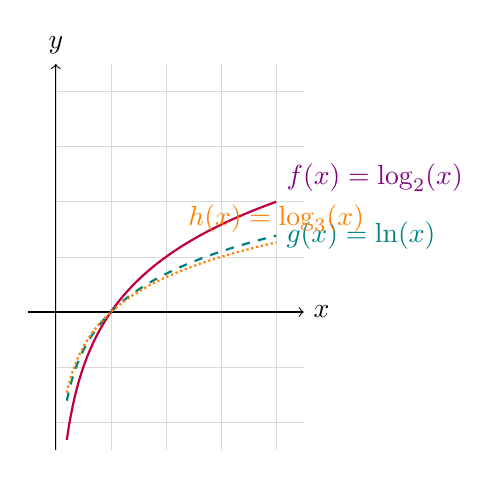
\begin{tikzpicture}[scale=0.7]
        % Grid
        \draw[step=1cm,gray,very thin,opacity=0.3] (0, -2.5) grid (4.5,4.5);

        % Axes
        \draw[->] (0,-2.5) -- (0,4.5) node[above] {$y$};
        \draw[->] (-0.5,0) -- (4.5,0) node[right] {$x$};

        % f(x) = log_2(x)
        \draw[thick,purple,domain=0.2:4,samples=100] plot(\x,{ln(\x)/ln(2)}) node[above right] {\textcolor{violet}{$f(x) = \log_2(x)$}};
        
        % g(x) = ln(x)
        \draw[thick,teal,dashed,domain=0.2:4,samples=100] plot(\x,{ln(\x)}) node[right] {\textcolor{teal}{$g(x) = \ln(x)$}};

        % h(x) = log_3(x)
        \draw[thick,orange,densely dotted,domain=0.2:4,samples=100] plot(\x,{ln(\x)/ln(3)}) node[above] {\textcolor{orange}{$h(x) = \log_3(x)$}};
      \end{tikzpicture}
    \end{column}

    % Right column: derivatives
    \begin{column}{0.5\textwidth}
      \centering
      \textbf{도함수들}

      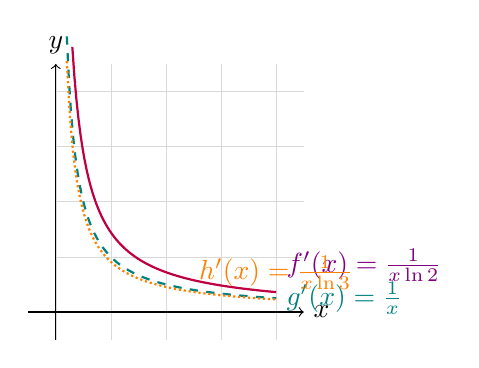
\begin{tikzpicture}[scale=0.7]
        % Grid
        \draw[step=1cm,gray,very thin,opacity=0.3] (0, -0.5) grid (4.5,4.5);

        % Axes
        \draw[->] (0,-0.5) -- (0,4.5) node[above] {$y$};
        \draw[->] (-0.5,0) -- (4.5,0) node[right] {$x$};

        % f'(x) = 1/(x ln2)
        \draw[thick,purple,domain=0.3:4,samples=100] plot(\x,{1/(\x*ln(2))}) node[above right] {\textcolor{violet}{$f'(x) = \frac{1}{x\ln 2}$}};
        
        % g'(x) = 1/x
        \draw[thick,teal,dashed,domain=0.2:4,samples=100] plot(\x,{1/\x}) node[right] {\textcolor{teal}{$g'(x) = \frac{1}{x}$}};

        % h'(x) = 1/(x ln3)
        \draw[thick,orange,densely dotted,domain=0.2:4,samples=100] plot(\x,{1/(\x*ln(3))}) node[above] {\textcolor{orange}{$h'(x) = \frac{1}{x\ln 3}$}};
      \end{tikzpicture}
    \end{column}
  \end{columns}
\end{frame}


\begin{frame}
  \begin{align*}
    & f(x) = \ln x^3     & f'(x)= \hspace{4cm} & f''(x)= \hspace{4cm} \\[2em]
    & f(x) = \log_{10} x & f'(x)= \hspace{4cm} & f''(x)= \hspace{4cm}
  \end{align*}
\end{frame}




\section{Product Rule}

\begin{frame}{곱의 미분}
  \begin{block}{곱의 미분법(= 나눗셈의 미분법)}
    \begin{align*}
      (f \cdot g)' = f' \cdot g + f \cdot g' \\
      \left(\frac{f}{g} \right)' = \frac{f' \cdot g - f \cdot g'}{g^2}
    \end{align*}
  \end{block}
\end{frame}


\begin{frame}{곱의 미분}
  \scalebox{0.85}{%
  \parbox{\linewidth}{%
  \begin{align*}
    & \text{함수 } \textcolor{blue}{f(x)}, \textcolor{red}{g(x)} \text{ 에 대해 } h(x) = \textcolor{blue}{f(x)}\textcolor{red}{g(x)} \text{ 라 하자} \\
    & h'(x) = \lim_{h \to 0} \frac{\textcolor{blue}{f(x+h)}\textcolor{red}{g(x+h)} - \textcolor{blue}{f(x)}\textcolor{red}{g(x)}}{h} \\
    \\
    & \textcolor{gray}{\text{두 항의 차를 직접 다루기 어렵기 때문에, 더하고 빼기}} \\
    & = \lim_{h \to 0} \frac{\textcolor{blue}{f(x+h)}\textcolor{red}{g(x+h)} - \textcolor{blue}{f(x)}\textcolor{red}{g(x+h)} + \textcolor{blue}{f(x)}\textcolor{red}{g(x+h)} - \textcolor{blue}{f(x)}\textcolor{red}{g(x)}}{h} \\
    & = \lim_{h \to 0} \left[ \frac{\textcolor{blue}{f(x+h)} - \textcolor{blue}{f(x)}}{h} \cdot \textcolor{red}{g(x+h)} + \textcolor{blue}{f(x)} \cdot \frac{\textcolor{red}{g(x+h)} - \textcolor{red}{g(x)}}{h} \right] \\
    \\
    & \text{극한은 각각 따로 가능하므로:} \\
    & = \left( \lim_{h \to 0} \frac{\textcolor{blue}{f(x+h)} - \textcolor{blue}{f(x)}}{h} \right) \cdot \left( \lim_{h \to 0} \textcolor{red}{g(x+h)} \right) + \textcolor{blue}{f(x)} \cdot \left( \lim_{h \to 0} \frac{\textcolor{red}{g(x+h)} - \textcolor{red}{g(x)}}{h} \right) \\
    & = \textcolor{blue}{f'(x)} \cdot \textcolor{red}{g(x)} + \textcolor{blue}{f(x)} \cdot \textcolor{red}{g'(x)} \\
    \\
    & \therefore \boxed{(\textcolor{blue}{f} \cdot \textcolor{red}{g})'(x) = \textcolor{blue}{f'(x)}\textcolor{red}{g(x)} + \textcolor{blue}{f(x)}\textcolor{red}{g'(x)}}
  \end{align*}
  }%
  }
\end{frame}

\begin{frame}
  \begin{align*}
    % & f(x) = x^2 + x \\
    %     & g(x) = a \cdot x^{10} + b \cdot x^5 + c \cdot x^2 + d \\
    %     & (f(x) \cdot g(x))' = \\
    & f(x) = x^2 + x ,  \quad g(x) = a \cdot x^{10} + b \cdot x^5 + c \cdot x^2 + d \\[1em]
    & \left(  f(x) \cdot g(x) \right)' =  \\[3em]
    & \left(  \frac{g(x)}{f(x)} \right)' =
    % & f(x) = x^2 + x     & f'(x)= \hspace{4cm} & f''(x)= \hspace{4cm} \\[2em]
    % & f(x) = x^2 + x     & f'(x)= \hspace{4cm} & f''(x)= \hspace{4cm} \\[2em]
    % & f(x) = \log_{10} x & f'(x)= \hspace{4cm} & f''(x)= \hspace{4cm}
  \end{align*}
\end{frame}








\section{Chain Rule}
% Chain rule.
\begin{frame}{주요 함수형태와 Chain Rule}
  \begin{block}{Chain Rule}
    \begin{align*}
      & h = {f} \circ {g} \text{ 인 합성함수 } h \text{ 라면} \\
      & h' = \mathbf{d} h  = ( {f} \circ {g} )' = {f'}({g}) \cdot {g'}
      % & \text{e.g. } h = {f} \circ {g} = f(g(x)) \\
      % & \frac{\mathbf{d}}{\mathbf{d}x} h = \frac{\mathbf{d}}{\mathbf{d}x} f(g(x)) = \frac{\mathbf{d}}{\mathbf{d}g(x)} f(g(x)) \cdot \frac{\mathbf{d}}{\mathbf{d}x} g(x) \\
      % & \text{이때, } u = g(x) \text{ 로 치환하면, 편리해 짐. 'u-substitution'이라는 미분 테크닉.} \\
      % & \text{e.g. } u = g(x) \rightarrow h = {f} \circ {g} = f(u), \quad  \\
      % & \frac{\mathbf{d}}{\mathbf{d}x} h = \frac{\mathbf{d}}{\mathbf{d}x} f(u) = \frac{\mathbf{d}}{\mathbf{d}u} f(u) \cdot \frac{\mathbf{d}u}{\mathbf{d}x}  \\
    \end{align*}
  \end{block}
  \begin{itemize}
    \item polynomial $ x $ polynomial: $ f(x) = (ax^2 + bx)^{c} $
    \item exponential $ x $ polynomial: $ g(x) = e^{ax^2 + bx + c} $
    \item logarithm $ x $ polynomial: $ h(x) = \ln (ax + b)^c $
  \end{itemize}
  
\end{frame}



\begin{frame}{합성함수의 미분: Chain Rule}
  \scalebox{0.85}{%
  \parbox{\linewidth}{%
  \begin{align*}
    % & \text{합성함수 } h(x) = \textcolor{blue}{f(}\textcolor{red}{g(x)}\textcolor{blue}{)} \text{ 에 대해 도함수를 정의로 구함} \\
    & h'(x) = \lim_{h \to 0} \frac{\textcolor{blue}{f(}\textcolor{red}{g(x+h)}\textcolor{blue}{)} - \textcolor{blue}{f(}\textcolor{red}{g(x)}\textcolor{blue}{)}}{h} \\
    % \\
    % & \textcolor{gray}{\text{(중간 단계: 분모에 } \textcolor{red}{g(x+h) - g(x)} \textcolor{gray}{ 를 곱하고 나누기)}} \\
    & = \lim_{h \to 0} \left[ \frac{\textcolor{blue}{f(}\textcolor{red}{g(x+h)}\textcolor{blue}{)} - \textcolor{blue}{f(}\textcolor{red}{g(x)}\textcolor{blue}{)}}{\textcolor{red}{g(x+h) - g(x)}} \cdot \frac{\textcolor{red}{g(x+h) - g(x)}}{h} \right] \\
    & \text{앞부분은 마치 } \frac{\Delta f(g(x))}{\Delta g(x)} \text{ 인데 $\Delta \to 0 $ 이면 미분의 정의} \\
    & \text{극한을 각각 분리하고, u를 치환하면:} \\
    % & \textcolor{gray}{\text{복잡한 함수의 극한을 다루기 위해 다음과 같이 치환한다:}} \\
    & \textcolor{black}{u = g(x+h)} \quad \Rightarrow \quad \textcolor{black}{u \to g(x)} \text{ as } h \to 0 \text{ (왜냐하면 } \textcolor{black}{g} \text{ 가 연속이므로)} \\
    & = \left( \lim_{\textcolor{red}{u} \to \textcolor{red}{g(x)}} \frac{\textcolor{blue}{f(}\textcolor{red}{u}\textcolor{blue}{)} - \textcolor{blue}{f(}\textcolor{red}{g(x)}\textcolor{blue}{)}}{\textcolor{red}{u - g(x)}} \right) \cdot \left( \lim_{h \to 0} \frac{\textcolor{red}{g(x+h)} - \textcolor{red}{g(x)}}{h} \right) \\
    & = \textcolor{blue}{f'}(\textcolor{red}{g(x)}) \cdot \textcolor{red}{g'(x)} \\
    % \\
    % & \therefore \boxed{( \textcolor{blue}{f} \circ \textcolor{red}{g} )'(x) = \textcolor{blue}{f'}(\textcolor{red}{g(x)}) \cdot \textcolor{red}{g'(x)}}
  \end{align*}
  }%
  }
\end{frame}








% Chain rule.
\begin{frame}{주요 함수형태와 Chain Rule}
  \begin{itemize}
    \item polynomial $ x $ polynomial : $ f(x) = (ax^2 + bx)^{c} $
        \begin{align*}
          f(x) & = (ax + b)^{-1}            & f'(x)= \hspace{5cm} \\
                                           && f''(x) = \hspace{5cm} \\
          f(x) & = (ax + b)^{20}            & f'(x)= \hspace{5cm} \\
                                           && f''(x) = \hspace{5cm} \\
          f(x) & = (ax^2 + bx + c)^{20}     & f'(x)= \hspace{5cm} \\
                                           && f''(x) = \hspace{5cm} \\
          f(x) & = a(2x+2)^2 + b(2x+2) + c  & f'(x)= \hspace{5cm} \\[1em]
          f(x) & = (ax+b)(cx+d)             & f'(x)= \hspace{5cm} 
        \end{align*}
    % \item exponential $ x $ polynomial
    % \item logarithm $ x $ polynomial
  \end{itemize}
  
\end{frame}

% Chain rule.
\begin{frame}{주요 함수형태와 Chain Rule}
  \begin{itemize}
    % \item polynomial $ x $ polynomial 
    \item exponential $ x $ polynomial : $ g(x) = e^{ax^2 + bx + c} $
      \begin{align*}
         g(x) & = e^{ax+b}                  & g'(x) = \hspace{6cm}  \\[1em]
         g(x) & = a^{bx+c}                  & g'(x) = \hspace{6cm}  \\[1em]
         g(x) & = e^{ax^2+bx+c}             & g'(x) = \hspace{6cm}  \\[1em]
         g(x) & = (ax+b)e^{cx+d}            & g'(x) = \hspace{6cm}  \\[1em]
         g(x) & = e^{ax+b}e^{cx+d}          & g'(x) = \hspace{6cm}  \\[1em]
         g(x) & = \frac{e^{ax+b}}{a^{cx+d}} & g'(x) = \hspace{6cm}   
      \end{align*}
    % \item logarithm $ x $ polynomial
  \end{itemize}
  
\end{frame}

% Chain rule.
\begin{frame}{주요 함수형태와 Chain Rule}
  \begin{itemize}
    \item logarithm $ x $ polynomial : $ h(x) = \ln (ax + b)^c $
      \begin{align*}
        & h(x) = \ln (ax + b)^{20}          & h'(x) = \hspace{6cm} \\[1em]
        & h(x) = \ln \frac{ax+b}{cx+d}      & h'(x) = \hspace{6cm} \\[1em]
        & h(x) = \frac{\ln ax+b}{\ln cx+d}  & h'(x) = \hspace{6cm} \\[1em]
        & h(x) = \log_{cx+d} (ax+b)         & h'(x) = \hspace{6cm}    
      \end{align*}
  \end{itemize}
  
\end{frame}



\section{미분가능}

\begin{frame}{연속성과 미분 가능성}
  \begin{block}{함수의 미분가능성}
    \begin{itemize}
      \item 함수 \( f(x) \)가 \( x = a \) 에서 미분 가능하려면, a에서 미분계수가 존재해야 함 :
      \[f'(a) = \lim_{h \to 0} \frac{f(a+h)-f(a)}{h} \quad \text{존재해야 함}\]
      \item 미분 가능성은 \textit{연속성을 포함}.
      \item 연속성이 있다고 해서 \textit{항상 미분 가능하진 않음}.
    \end{itemize}
  \end{block}
  \begin{block}{함수의 연속성}
    \begin{itemize}
      \item 함수 \( f(x) \)가 \( x = a \) 에서 연속이려면, a 에서 함수값과 함수의 극한값이 동일해야 함 :
      \[\lim_{x \to a} f(x) = f(a)\]
    \end{itemize}
  \end{block}
\end{frame}





\section{역함수의 미분법}

% Inverse function.
\begin{frame}{역함수의 미분법칙 (Inverse-Function Rule)}
  % \scriptsize
    \textbf{역함수 존재 조건:}
    \begin{itemize}
      \item \( y = f(x) \) 가 일대일 대응(one-to-one mapping)이면, 역함수 \( x = f^{-1}(y) \) 존재.
      \item 함수 \( f(x) \)가 \textbf{strictly monotonic} (엄격히 단조 증가 또는 감소)이면 역함수 존재.
      \item 단조성 확인법: \( f'(x) \)가 모든 구간에서 부호가 일정하고 \( f'(x) \neq 0 \).
      \item \( y = f(x) \)와 \( x = f^{-1}(y) \) 그래프는 \( y=x \) 대각선을 기준으로 대칭.
    \end{itemize}
    % 
  \begin{block}{역함수 미분법 (Inverse-Function Differentiation Rule)}
    원 함수의 도함수와 역함수의 도함수는 \textbf{서로 역수 관계}
    \begin{align*}
      \frac{dx}{dy} = \frac{1}{\frac{dy}{dx}}
    \end{align*}
  \end{block}
\end{frame}



\begin{frame}{역함수 미분법 예시: 완전대체재 수요함수}
  \scriptsize
  \begin{columns}
    % Left column: Graph
    \begin{column}{0.5\textwidth}
      \centering
      \textbf{수요함수와 역수요함수 관계}

      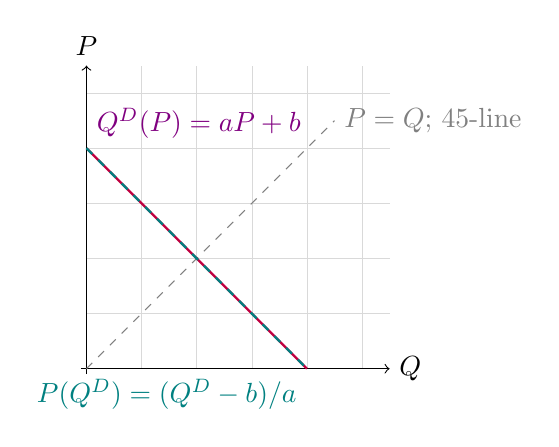
\begin{tikzpicture}[scale=0.7]
        % Grid
        \draw[step=1cm,gray,very thin,opacity=0.3] (0,0) grid (5.5,5.5);

        % Axes
        \draw[->] (-0.1,0) -- (5.5,0) node[right] {$Q$};
        \draw[->] (0,-0.1) -- (0,5.5) node[above] {$P$};

        % 45 degree line
        \draw[dashed,gray] (-0.0,-0.0) -- (4.5,4.5) node[right] {$P=Q$; 45-line};

        % Q^d(P) curve
        \draw[thick,purple,domain=0:4,samples=100] plot({(-\x+4)},\x) node[above right] {\textcolor{violet}{$Q^D(P) = aP+b$}};

        % Inverse demand P(Q)
        \draw[thick,teal,dashed,domain=0:4,samples=100] plot(\x,{(-\x+4)}) node[below left] {\textcolor{teal}{$P(Q^D) = (Q^D-b)/a$}};
      \end{tikzpicture}
    \end{column}

    % Right column: Derivative relationships
    \begin{column}{0.5\textwidth}
      \centering
      \scalebox{0.85}{
      \begin{minipage}{\textwidth}
      \textbf{도함수 관계}

      \vspace{1em}

      \begin{itemize}
        \item \textbf{수요함수:}
        \[
        Q^D(P) = aP+b
        \quad (a<0)
        \]
        \[
        \frac{\mathbf{d}Q^D}{\mathbf{d}P} = a
        \]
        \item \textbf{역수요함수:}
        \[
        P(Q^D) = \frac{Q^D-b}{a}
        \quad \Rightarrow \quad
        \frac{\mathbf{d}P}{\mathbf{d}Q^D} = \frac{1}{a}
        \]
        \item \textbf{Inverse-Function Rule:}
        \[
        \frac{\mathbf{d}P}{\mathbf{d}Q^D} = \frac{1}{\frac{\mathbf{d}Q^D}{\mathbf{d}P}}
        \quad \text{(역수 관계)}
        \]
        \item \( a<0 \) 이므로:
        \[
        \frac{\mathbf{d}P}{\mathbf{d}Q^D} < 0
        \]
      \end{itemize}
      \end{minipage}
      }
    \end{column}
  \end{columns}
\end{frame}


\begin{frame}{역함수 미분법 예시: Cobb-Douglas 형태 수요함수}
  \scriptsize
  \begin{columns}
    % Left column: Graph
    \begin{column}{0.4\textwidth}
      \centering
      \textbf{수요함수와 역수요함수 관계}

      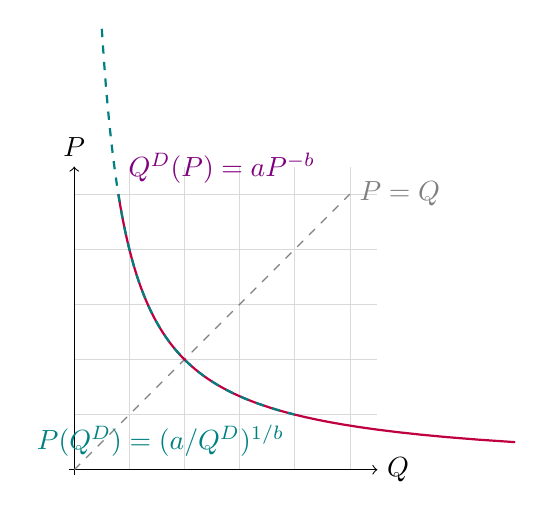
\begin{tikzpicture}[scale=0.7]
        % Grid
        \draw[step=1cm,gray,very thin,opacity=0.3] (0,0) grid (5.5,5.5);

        % Axes
        \draw[->] (-0.1,0) -- (5.5,0) node[right] {$Q$};
        \draw[->] (0,-0.1) -- (0,5.5) node[above] {$P$};

        % 45 degree line
        \draw[dashed,gray] (0,0) -- (5,5) node[right] {$P=Q$};

        % Q^D(P) curve
        \draw[thick,purple,domain=0.5:5,samples=100] plot({4/(\x)},\x) node[above right] {\textcolor{violet}{$Q^D(P) = aP^{-b}$}};

        % Inverse demand P(Q^D)
        \draw[thick,teal,dashed,domain=0.5:4,samples=100] plot(\x,{4/(\x)}) node[below left] {\textcolor{teal}{$P(Q^D) = (a/Q^D)^{1/b}$}};
      \end{tikzpicture}
    \end{column}

    % Right column: Derivative relationships
    \begin{column}{0.6\textwidth}
      \centering
      \scalebox{0.85}{
      \begin{minipage}{\textwidth}
      \textbf{도함수 관계}

      \vspace{1em}

      \begin{itemize}
        \item \textbf{수요함수:}
        \[
        Q^D(P) = aP^{-b}
        \quad (a>0, b>0)
        \]
        \[
        \frac{\mathbf{d}Q^D}{\mathbf{d}P} = -abP^{-(b+1)}
        \]
        \item \textbf{역수요함수:}
        \[
        P(Q^D) = \left(\frac{a}{Q^D}\right)^{1/b}
        \quad \Rightarrow \quad
        \frac{\mathbf{d}P}{\mathbf{d}Q^D} = -\frac{1}{b}\left(\frac{a}{Q^D}\right)^{1/b} \frac{1}{Q^D}
        \]
        \item \textbf{Inverse-Function Rule:}
        \[
        \frac{\mathbf{d}P}{\mathbf{d}Q^D} = \frac{1}{\frac{\mathbf{d}Q^D}{\mathbf{d}P}}
        \quad \text{(역수 관계)}
        \]
        \item \( b>0 \) 이므로:
        \[
        \frac{\mathbf{d}P}{\mathbf{d}Q^D} < 0
        \]
      \end{itemize}
      \end{minipage}
      }
    \end{column}
  \end{columns}
\end{frame}


\begin{frame}
  \begin{align*}
    & f(x) = x ,  \quad f^{-1}(x) = 1/x \\[1em]
    & f'(x) =  \\[1em]
    & \left(  f^{-1}(x) \right)' = \\[2em]
    & g(x) = e^x ,  \quad g^{-1}(x) = \ln x \\[1em]
    & g'(x) =  \\[1em]
    & \left(  g^{-1}(x) \right)' = 
  \end{align*}
\end{frame}




\section{미분법칙 정리}

\begin{frame}{미분법칙 요약}
  \scalebox{0.85}{%
  \parbox{\linewidth}{%
    \begin{align*}
      \text{Constant Rule: } & \frac{\mathbf{d}}{\mathbf{d}x} c = 0 \\[1em]
      \text{Power Rule: } & \frac{\mathbf{d}}{\mathbf{d}x} x^n = n \cdot x^{n-1} \\[1em]
      \text{Exponential Rule: } & \frac{d}{dx} e^x = e^x  \\
                                & \frac{d}{dx} a^x = a^x \cdot \ln a \\[1em]
      \text{Logarithm Rule: } & \frac{d}{dx} \ln x = \frac{1}{x} \\
                              & \frac{d}{dx} \log_a x = \frac{1}{x \ln a}
    \end{align*}
    }%
    }
\end{frame}

\begin{frame}{미분법칙 요약}
  \scalebox{0.85}{%
  \parbox{\linewidth}{%
    \begin{align*}
      \text{Sum-Diff Rule: } & \frac{\mathbf{d}}{\mathbf{d}x} [f(x) \pm g(x)] = \frac{\mathbf{d}}{\mathbf{d}x} f(x) \pm \frac{\mathbf{d}}{\mathbf{d}x} g(x) \\[1em]
      \text{Product Rule: } & \frac{\mathbf{d}}{\mathbf{d}x}[f(x) \cdot g(x)] = \frac{\mathbf{d}}{\mathbf{d}x} f(x) \cdot g(x) + f(x) \cdot \frac{\mathbf{d}}{\mathbf{d}x} g(x) \\[1em]
      \text{Quotient Rule: } & \frac{\mathbf{d}}{\mathbf{d}x}  \frac{f(x)}{g(x)}   = \frac{ \frac{\mathbf{d}}{\mathbf{d}x} f(x) \cdot g(x) - f(x) \cdot \frac{\mathbf{d}}{\mathbf{d}x} g(x)}{{g(x)}^2} \\[1em]
      \text{Chain Rule: } & h=f(y), \, y=g(x) \text{ then } \frac{\mathbf{d}}{\mathbf{d}x} h(y)  = \frac{\mathbf{d}}{\mathbf{d}x} f(g(x)) = \frac{\mathbf{d}}{\mathbf{d}y} f(y) \cdot \frac{\mathbf{d}}{\mathbf{d}x} g(x) \\[1em]
      \text{Inverse-Function Rule: } & If \, y=f(x) \, and \, f^{-1}(y) = x \, exists, \, \text{then the differentiation for the inverse function: } \\[1em]
      & \frac{\mathbf{d}}{\mathbf{d}y} x = \frac{1}{\frac{\mathbf{d}}{\mathbf{d}x} y} \Leftrightarrow \frac{\mathbf{d}x}{\mathbf{d}y} = \frac{1}{\frac{\mathbf{d}y}{\mathbf{d}x}}
    \end{align*}
    }%
    }
\end{frame}


\begin{frame}{미분법칙 요약 (Simplified)}
  \scalebox{0.85}{%
  \parbox{\linewidth}{%
    \begin{align*}
      \text{Sum-Diff Rule: } & (f \pm g)' = f' \pm g' \\[1em]
      \text{Product Rule: } & (f \cdot g)' = f'\cdot g + f\cdot g' \\[1em]
      \text{Quotient Rule: } &   \left(   \frac{f}{g} \right)'  = \frac{  f' \cdot g - f \cdot  g'}{g^2} \\[1em]
      \text{Chain Rule: } &  \left(f(g(\cdot))\right)' = f'(g(\cdot))\cdot g'(\cdot) \\[1em]
      \text{Inverse-Function Rule: } & \left( f^{-1} \right)' = \frac{1}{f'}
    \end{align*}
    }%
    }
\end{frame}





%%%%%%%%%%%%%%%%%%%%%%%%%%%%%%%%%%%%%
%%%%%%%%%%%%%%%%%%%%%%%%%%%%%%%%%%%%%
% 
% 도함수
%  
%%%%%%%%%%%%%%%%%%%%%%%%%%%%%%%%%%%%%
%%%%%%%%%%%%%%%%%%%%%%%%%%%%%%%%%%%%%







% %%%%%%%%%%%%%%%%%%%%%%%%%%%%%%%%%%%%%
% %%%%%%%%%%%%%%%%%%%%%%%%%%%%%%%%%%%%%
% % 
% % 미분형 (더욱추상적)
% %  
% %%%%%%%%%%%%%%%%%%%%%%%%%%%%%%%%%%%%%
% %%%%%%%%%%%%%%%%%%%%%%%%%%%%%%%%%%%%%

% \section{편미분 Partial Differentiation}

% % 편미분
% \begin{frame}{편미분: Partial Differentiation}
%   \scriptsize
%   \begin{columns}
%     % Left column: Explanation
%     \begin{column}{0.5\textwidth}
%       \centering
%       \textbf{Partial Differentiation 개념}

%       \vspace{0.5em}

%       \begin{itemize}
%         \item 다변수 함수:
%         \[
%         y = f(x_1, x_2, \dots, x_n)
%         \]
%         \item \textbf{Partial Derivative}:  
%         한 변수만 변하게 하고, 나머지는 고정하여 미분.
%         \[
%         \frac{\partial y}{\partial x_i} = \lim_{\Delta x_i \to 0} \frac{f(x_1, \dots, x_i + \Delta x_i, \dots, x_n) - f(x_1, \dots, x_n)}{\Delta x_i}
%         \]
%         \item 표기법:
%         \[
%         \frac{\partial y}{\partial x_i}, \quad \frac{\partial f}{\partial x_i}, \quad f_i
%         \]
%         \item 주의: 편미분 시 \((n-1)\) 개 변수는 상수 취급
%       \end{itemize}
%     \end{column}

%     % Right column: Example
%     \begin{column}{0.5\textwidth}
%       \centering
%       \textbf{예제: 부분 미분}

%       \vspace{0.5em}

%       주어진 함수:
%       \[
%       y = 3x_1^2 + x_1x_2 + 4x_2^2
%       \]

%       \vspace{0.5em}

%       \textbf{Partial derivatives:}
%       \[
%       \frac{\partial y}{\partial x_1} = 6x_1 + x_2
%       \]
%       \[
%       \frac{\partial y}{\partial x_2} = x_1 + 8x_2
%       \]

%       \vspace{0.5em}

%       \textbf{특정 점에서 계산:} \((x_1, x_2) = (1,3)\)
%       \[
%       f_1(1,3) = 6(1) + 3 = 9
%       \]
%       \[
%       f_2(1,3) = 1 + 8(3) = 25
%       \]
%     \end{column}
%   \end{columns}
% \end{frame}





% % 비교정태분석
% \begin{frame}{비교정태 분석: Comparative-Static Analysis}
%   \scriptsize
%   \begin{columns}
%     % Left column: Concept
%     \begin{column}{0.5\textwidth}
%       \centering
%       \textbf{비교정태 분석 개념}

%       \vspace{0.5em}

%       \begin{itemize}
%         \item \textbf{목적:}  
%         외생변수(exogenous variable)의 변화가 내생변수(endogenous variable)에 미치는 영향을 분석
%         \item \textbf{방법:}  
%         - 균형값(equilibrium value)을 외생변수에 대해 편미분
%         \item \textbf{수식 예시 (Reduced Form):}
%         \[
%         P^* = \frac{a+c}{b+d}, \quad Q^* = \frac{ad-bc}{b+d}
%         \]
%         \item \textbf{비교정태 도함수 (Comparative-Static Derivatives):}
%         \[
%         \frac{\partial P^*}{\partial a}, \quad \frac{\partial P^*}{\partial b}, \quad \frac{\partial P^*}{\partial c}, \quad \frac{\partial P^*}{\partial d}
%         \]
%       \end{itemize}
%     \end{column}

%     % Right column: Example
%     \begin{column}{0.5\textwidth}
%       \centering
%       \textbf{시장모형 예시}

%       \vspace{0.5em}

%       수요: \( Q = a - bP \quad (a, b>0) \)\\
%       공급: \( Q = -c + dP \quad (c, d>0) \)

%       \vspace{0.5em}

%       \textbf{P*에 대한 편미분 결과:}
%       \[
%       \frac{\partial P^*}{\partial a} = \frac{1}{b+d} > 0
%       \quad
%       \frac{\partial P^*}{\partial c} = \frac{1}{b+d} > 0
%       \]
%       \[
%       \frac{\partial P^*}{\partial b} = \frac{-(a+c)}{(b+d)^2} < 0
%       \quad
%       \frac{\partial P^*}{\partial d} = \frac{-(a+c)}{(b+d)^2} < 0
%       \]

%       \vspace{0.5em}

%       \textbf{해석:}
%       \begin{itemize}
%         \item \( a \) 또는 \( c \) 증가 → \( P^* \) 증가
%         \item \( b \) 또는 \( d \) 증가 → \( P^* \) 감소
%       \end{itemize}
%     \end{column}
%   \end{columns}
% \end{frame}





% % 자코비안
% \begin{frame}{Jacobian Determinant: 자코비안 행렬식}
%   \scriptsize
%   \begin{columns}
%     % Left column: Concept
%     \begin{column}{0.5\textwidth}
%       \centering
%       \textbf{Jacobian 개념}

%       \vspace{0.5em}

%       \begin{itemize}
%         \item \textbf{정의:}  
%         여러 변수에 대한 함수들의 편미분을 모아 만든 행렬의 행렬식
%         \[
%         |J| = \frac{\partial(y_1, \dots, y_n)}{\partial(x_1, \dots, x_n)}
%         \]
%         \item \textbf{형태:}
%         \[
%         J =
%         \begin{bmatrix}
%           \frac{\partial y_1}{\partial x_1} & \cdots & \frac{\partial y_1}{\partial x_n} \\
%           \vdots & \ddots & \vdots \\
%           \frac{\partial y_n}{\partial x_1} & \cdots & \frac{\partial y_n}{\partial x_n}
%         \end{bmatrix}
%         \]
%         \item \textbf{Jacobian 판별법:}
%         \begin{itemize}
%           \item \( |J| = 0 \) : 함수들 사이에 종속성 존재
%           \item \( |J| \neq 0 \) : 독립적
%         \end{itemize}
%       \end{itemize}
%     \end{column}

%     % Right column: Example
%     \begin{column}{0.5\textwidth}
%       \centering
%       \textbf{예제: 두 함수의 Jacobian}

%       \vspace{0.5em}

%       주어진 함수:
%       \[
%       y_1 = 2x_1 + 3x_2,\quad
%       y_2 = 4x_1^2 + 12x_1x_2 + 9x_2^2
%       \]

%       편미분 결과:
%       \[
%       \frac{\partial y_1}{\partial x_1} = 2, \quad \frac{\partial y_1}{\partial x_2} = 3
%       \]
%       \[
%       \frac{\partial y_2}{\partial x_1} = 8x_1 + 12x_2, \quad \frac{\partial y_2}{\partial x_2} = 12x_1 + 18x_2
%       \]

%       Jacobian 계산:
%       \[
%       |J| = 2(12x_1 + 18x_2) - 3(8x_1 + 12x_2) = 0
%       \]

%       \textbf{결론:} \( y_1, y_2 \) 는 종속적 (ex: \( y_2 = y_1^2 \))
%     \end{column}
%   \end{columns}
% \end{frame}





% \section{미분형과 도함수와 미분}
% %%%%%%%%%%%%%%%%%%%%%%%%%%%%%%%%%%%%%
% % Sec. Differentials and Derivatives.
% %%%%%%%%%%%%%%%%%%%%%%%%%%%%%%%%%%%%%
% \begin{frame}{미분형형과 도함수: Differentials and Derivatives}
%   \scriptsize
%   \begin{columns}
%     % Left column: Concept
%     \begin{column}{0.5\textwidth}
%       \centering
%       \textbf{개념 설명}

%       \vspace{0.5em}

%       \begin{itemize}
%         \item 전통적 해석: \( \frac{dy}{dx} \) 는 하나의 기호
%         \item 새로운 해석:  
%           - \( dy \) 와 \( dx \) 두 양의 비율로 분리
%           - \[
%             \frac{dy}{dx} = \lim_{\Delta x \to 0} \frac{\Delta y}{\Delta x}
%             \]
%         \item \textbf{차이:}
%           - \( \Delta y \approx f(x) \Delta x + \delta \Delta x \)
%           - \( dy = f(x) dx \) (오차항 무시)
%         \item \textbf{의미:}
%           - \( dx \): 독립변수의 변화량
%           - \( dy \): 종속변수의 근사 변화량
%           - \( f(x) \) 는 "변환기(converter)" 역할
%       \end{itemize}
%     \end{column}

%     % Right column: Example
%     \begin{column}{0.5\textwidth}
%       \centering
%       \textbf{수식과 예시}

%       \vspace{0.5em}

%       그래프 해석:

%       \begin{itemize}
%         \item \( \Delta y \) : 실제 변화량 (곡선 이동)
%         \item \( dy \) : 접선에 따른 근사 변화량
%       \end{itemize}

%       \vspace{0.5em}

%       수식 관계:
%       \[
%       dy = f(x) dx
%       \]

%       \vspace{0.5em}

%       예시:

%       함수 \( y = x^2 \) 에 대해,
%       \[
%       f(x) = 2x
%       \]
%       따라서,
%       \[
%       dy = 2x \, dx
%       \]

%       \( x = 3 \), \( dx = 0.01 \) 일 때:
%       \[
%       dy = 2(3)(0.01) = 0.06
%       \]
%     \end{column}
%   \end{columns}
% \end{frame}



% % Slide 2: 그림과 예제
% \begin{frame}{Differentials and Derivatives: 그래픽 예시}
%   \scriptsize
%   \begin{columns}
%     \begin{column}{0.5\textwidth}
%       \textbf{그래프 설명}

%       \vspace{0.5em}
%       \begin{itemize}
%         \item \( x_0 \)에서 \( x_0 + \Delta x \)로 이동
%         \item 곡선 위 실제 변화: \( \Delta y \)
%         \item 접선 근사 변화: \( dy \)
%       \end{itemize}

%       \vspace{1em}
%       \[
%       dy = f'(x_0) dx
%       \quad
%       \Delta y \approx dy \quad (\text{when } dx \to 0)
%       \]
%     \end{column}
%     \begin{column}{0.5\textwidth}
%       \centering
%       % Simplified illustration
%       \begin{tikzpicture}[scale=0.7]
%         \draw[->] (-0.5,0) -- (4.5,0) node[right] {$x$};
%         \draw[->] (0,-0.5) -- (0,4.5) node[above] {$y$};

%         % curve
%         \draw[thick,blue,domain=0:4,samples=100] plot(\x,{0.5*\x*\x/2}) node[right] {$y=f(x)$};

%         % tangent at x0
%         \draw[dashed,red] (1,0.25) -- (3,2.25);

%         % points
%         \filldraw (1,0.25) circle (2pt) node[below left] {$A(x_0,y_0)$};
%         \filldraw (3,2.25) circle (2pt) node[below right] {$C(x_0+dx,y_0+dy)$};

%         \draw[decorate,decoration={brace,mirror,amplitude=8pt}] (1,0) -- (3,0) node[midway,below=8pt] {$dx$};
%         \draw[decorate,decoration={brace,amplitude=8pt}] (0,0.25) -- (0,2.25) node[midway,left=8pt] {$dy$};
%       \end{tikzpicture}
%     \end{column}
%   \end{columns}
% \end{frame}

% % Slide 3: 수학적 요약
% \begin{frame}{Differentials and Derivatives: 요약 및 개념적 포인트}
%   \scriptsize
%   \begin{itemize}
%     \item \textbf{Differential \( dx \)}:  
%     독립 변수의 변화 (任意로 설정 가능).
%     \item \textbf{Differential \( dy \)}:  
%     \( dx \)에 의해 유발되는 종속 변수의 근사 변화:
%     \[
%     dy = f'(x) dx
%     \]
%     \item \textbf{Derivative \( \frac{dy}{dx} \)}:  
%     두 differential 간의 비율로, \( x \)가 극소로 변할 때의 기울기.
%     \item \textbf{핵심 개념:}
%     \begin{itemize}
%       \item \( dy \)는 \( f'(x) \)와 \( dx \)에 종속.
%       \item \( dy \)는 독립적으로 존재하지 않고, 항상 어떤 \( dx \)와 짝지어 생각해야 한다.
%       \item \( dy = f'(x)dx \)는 "변환기"처럼 작용한다: \( dx \to dy \).
%     \end{itemize}
%   \end{itemize}
% \end{frame}





% \section{전미분형}
% %%%%%%%%%%%%%%%%%%%%%%%%%%%%%%%%%%%%%
% % Sec. Total Differentials (전미분형)
% %%%%%%%%%%%%%%%%%%%%%%%%%%%%%%%%%%%%%
% \begin{frame}{Total Differentials: 전체 미분}
%   \scriptsize
%   \begin{columns}
%     % Left column: Concept
%     \begin{column}{0.5\textwidth}
%       \centering
%       \textbf{개념 설명}

%       \vspace{0.5em}

%       \begin{itemize}
%         \item \textbf{정의:}  
%         다변수 함수의 전체 변화량을 근사하는 선형 결합
%         \[
%         dF = \sum_{i=1}^{n} \frac{\partial F}{\partial x_i} dx_i
%         \]
%         \item \textbf{기호:}
%         \[
%         dF = F_1 dx_1 + F_2 dx_2 + \cdots + F_n dx_n
%         \]
%         \item \textbf{의미:}
%         \begin{itemize}
%           \item 각 독립변수의 변화가 종속변수에 미치는 영향을 합산
%           \item \(\partial F / \partial x_i\) 는 "변환기"처럼 작용
%         \end{itemize}
%         \item \textbf{용어 정리:}
%         \begin{itemize}
%           \item \textbf{Total differential:} 전체 변화량 근사
%           \item \textbf{Partial differential:} 개별 독립변수의 영향
%         \end{itemize}
%       \end{itemize}
%     \end{column}

%     % Right column: Examples
%     \begin{column}{0.5\textwidth}
%       \centering
%       \textbf{예제: Saving 함수와 Utility 함수}

%       \vspace{0.5em}

%       \textbf{Saving function:}
%       \[
%       S = S(Y, i)
%       \]
%       \[
%       dS = \frac{\partial S}{\partial Y} dY + \frac{\partial S}{\partial i} di
%       \]
%       \[
%       dS = S_Y dY + S_i di
%       \]

%       \vspace{0.5em}

%       \textbf{Utility function:}
%       \[
%       U = U(x_1, x_2, \dots, x_n)
%       \]
%       \[
%       dU = \sum_{i=1}^{n} \frac{\partial U}{\partial x_i} dx_i
%       \]
%       \[
%       dU = U_1 dx_1 + U_2 dx_2 + \cdots + U_n dx_n
%       \]

%       \vspace{0.5em}

%       \textbf{경제적 해석:}
%       \begin{itemize}
%         \item \( S_Y dY \): 소득 변화에 의한 저축 변화
%         \item \( S_i di \): 이자율 변화에 의한 저축 변화
%       \end{itemize}
%     \end{column}
%   \end{columns}
% \end{frame}



% %%%%%%%%%%%%%%%%%%%%%%%%%%%%%%%%%%%%%
% % Sec. Rules of Differentials
% %%%%%%%%%%%%%%%%%%%%%%%%%%%%%%%%%%%%%

% \section{전도함수}
% %%%%%%%%%%%%%%%%%%%%%%%%%%%%%%%%%%%%%
% % Sec. Total Derivatives (전도함수)
% %%%%%%%%%%%%%%%%%%%%%%%%%%%%%%%%%%%%%
% \begin{frame}{Total Derivatives: 전체 도함수}
%   \scriptsize
%   \begin{columns}
%     % Left column: Concept
%     \begin{column}{0.5\textwidth}
%       \centering
%       \textbf{개념 설명}

%       \vspace{0.5em}

%       \begin{itemize}
%         \item \textbf{상황:}  
%         변수들이 서로 종속될 때, 전체 변화율을 구하는 방법
%       \item \textbf{구성:}
%         \[
%         y = f(x, w), \quad x = g(w)
%         \quad \Rightarrow \quad
%         y = f[g(w), w]
%         \]
%       \item \textbf{Total Derivative 공식:}
%         \[
%         \frac{dy}{dw} = \frac{\partial y}{\partial x} \frac{dx}{dw} + \frac{\partial y}{\partial w}
%         \]
%       \item \textbf{구조적 이해 (채널맵):}
%         \begin{itemize}
%           \item \( w \to x \to y \) (간접경로)
%           \item \( w \to y \) (직접경로)
%         \end{itemize}
%       \item \textbf{중요 구분:}
%         \[
%         \frac{dy}{dw} \quad (\text{Total}) \quad vs. \quad \frac{\partial y}{\partial w} \quad (\text{Partial})
%         \]
%       \end{itemize}
%     \end{column}

%     % Right column: Example
%     \begin{column}{0.5\textwidth}
%       \centering
%       \textbf{예제: 함수 관계 분석}

%       \vspace{0.5em}

%       \textbf{주어진 관계:}
%       \[
%       y = f(x,w), \quad x = g(w)
%       \]

%       전체 미분:
%       \[
%       dy = \frac{\partial y}{\partial x} dx + \frac{\partial y}{\partial w} dw
%       \]

%       \vspace{0.5em}

%       양변을 \( dw \)로 나누면:
%       \[
%       \frac{dy}{dw} = \frac{\partial y}{\partial x} \frac{dx}{dw} + \frac{\partial y}{\partial w}
%       \]

%       \vspace{0.5em}

%       \textbf{경제적 해석:}
%       \begin{itemize}
%         \item \( \partial y / \partial x \): x 변화가 y에 미치는 영향
%         \item \( dx/dw \): w 변화가 x에 미치는 영향
%         \item \( \partial y / \partial w \): w가 직접 y에 미치는 영향
%       \end{itemize}
%     \end{column}
%   \end{columns}
% \end{frame}


% \section{Implicit Function}
% %%%%%%%%%%%%%%%%%%%%%%%%%%%%%%%%%%%%%
% % Sec. Implicit function (경제학에서 제일 중요한 개념, 생산량에 따라)
% %%%%%%%%%%%%%%%%%%%%%%%%%%%%%%%%%%%%%
% % Slide 1: Implicit Functions
% \begin{frame}{Implicit Functions: 암시적 함수 (음함수)}
%   \scriptsize
%   \begin{itemize}
%     \item \textbf{Explicit function:}  
%     \[
%     y = f(x) \quad \text{(e.g., } y = 3x^4 \text{)}
%     \]
%     \item \textbf{Implicit function:}  
%     \[
%     F(y,x) = 0 \quad \text{(e.g., } y - 3x^4 = 0 \text{)}
%     \]
%     \item \textbf{특징:}
%     \begin{itemize}
%       \item \( y \)가 명시적으로 주어지지 않음
%       \item 관계식으로 \( y \)가 정의됨
%     \end{itemize}
%     \item \textbf{예시:}
%     \[
%     x^2 + y^2 = 9
%     \]
%     - 전체 원(circle)을 나타내는 관계.  
%     - \( y = +\sqrt{9-x^2} \) (상반부), \( y = -\sqrt{9-x^2} \) (하반부) 로 부분함수 가능.
%   \end{itemize}
% \end{frame}

% % Slide 2: Implicit Function Theorem
% \begin{frame}{Implicit Function Theorem}
%   \scriptsize
%   \begin{itemize}
%     \item \textbf{문제:}  
%     \[
%     F(y, x_1, \dots, x_m) = 0
%     \quad \Rightarrow \quad
%     y = f(x_1, \dots, x_m) \,?
%     \]
%     \item \textbf{조건:}
%     \begin{itemize}
%       \item \( F \)는 연속적이고, 부분 미분계수 \( F_y, F_1, \dots, F_m \) 존재
%       \item 특정 점에서 \( F_y \neq 0 \)
%     \end{itemize}
%     \item \textbf{결론:}
%     \begin{itemize}
%       \item 그 근방에서 \( y = f(x_1, \dots, x_m) \) 암시적 함수 존재
%       \item \( f \)는 연속적이며, 부분 미분가능
%     \end{itemize}
%     \item \textbf{예시:}
%     \[
%     x^2 + y^2 = 9
%     \quad \Rightarrow \quad
%     y = \pm \sqrt{9-x^2} \quad \text{(부분구간)}
%     \]
%     - \( F_y = 2y \neq 0 \)이면, 근방에 \( y=f(x) \) 존재
%   \end{itemize}
% \end{frame}

% % Slide 3: Derivatives of Implicit Functions
% \begin{frame}{Derivatives of Implicit Functions}
%   \scriptsize
%   \begin{itemize}
%     \item \textbf{방법:}
%     \[
%     dF = F_y dy + F_1 dx_1 + \cdots + F_m dx_m = 0
%     \]
%     \item \textbf{결론 (Implicit Function Rule):}
%     \[
%     \frac{\partial y}{\partial x_i} = -\frac{F_i}{F_y} \quad (i=1,2,\dots,m)
%     \]
%     \item \textbf{간단한 경우:}
%     \[
%     \frac{dy}{dx} = -\frac{F_x}{F_y}
%     \]
%     \item \textbf{예시:}
%     \[
%     F(y,x) = x^2 + y^2 - 9 = 0
%     \]
%     \[
%     F_y = 2y, \quad F_x = 2x
%     \quad \Rightarrow \quad
%     \frac{dy}{dx} = -\frac{2x}{2y} = -\frac{x}{y}
%     \]
%   \end{itemize}
% \end{frame}


% %%%%%%%%%%%%%%%%%%%%%%%%%%%%%%%%%%%%%
% % Sec. Comparative stastistics
% %%%%%%%%%%%%%%%%%%%%%%%%%%%%%%%%%%%%%



% \begin{frame}
  
% \end{frame}


\end{document}
